\section{Simulation Results}
\label{simulation}
    \begin{table}[ht]
    \label{parameter set}
    \center
    \begin{tabular}{|l|l|l|}
    \hline
    Parameter                       & Value  &                                       \\ \hline
    Number of devices               &20000 to 30000  & \multirow{6}{*}{~\cite{3GPP37.868}}   \\ \cline{1-2}
    Number of preambles             & 54     &                                       \\ \cline{1-2}
    Maximum allowable transmissions & 10     &                                       \\ \cline{1-2}
    Collision Backoff time          & 20 ms  &                                       \\ \cline{1-2}
    Arrival period                  & 10s    &                                       \\ \cline{1-2}
    PRACH Configuration Index       & 6      &                                       \\ \hline
    ACB Backoff time                & 320 ms &                                       \\ \hline
    ACB factor for group 1          & 1      &                                       \\ \hline
    ACB factor for group 2          & 1      &                                       \\ \hline
    \end{tabular}
    \end{table}

    In this section, we use Matlab to finish the work. Our parameter set is refered from~\cite{3GPP37.868} to make our model more practical. We examine the throughput performance of our proposed work and traditional methods for various settings of parameters values. There are different number of devices $N_{sys}$ that we simulate in our model, and it's range is from $20000$ to $30000$. Simulation will terminate if there are not any MTC devices in the system.
    \begin{figure}[t]
    \centering
    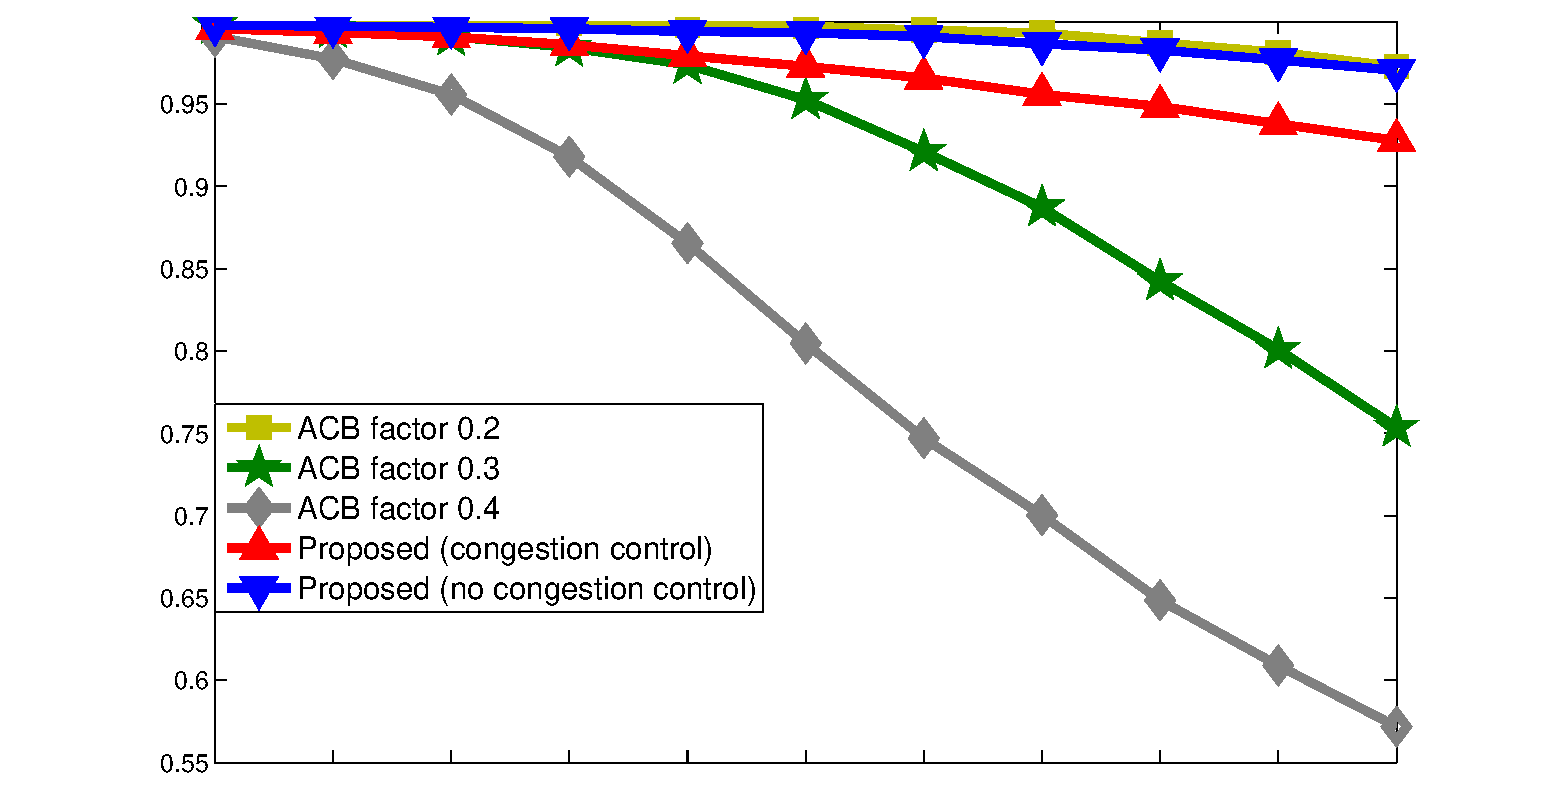
\includegraphics[width=3.8in]{combine_suc.eps}
    % 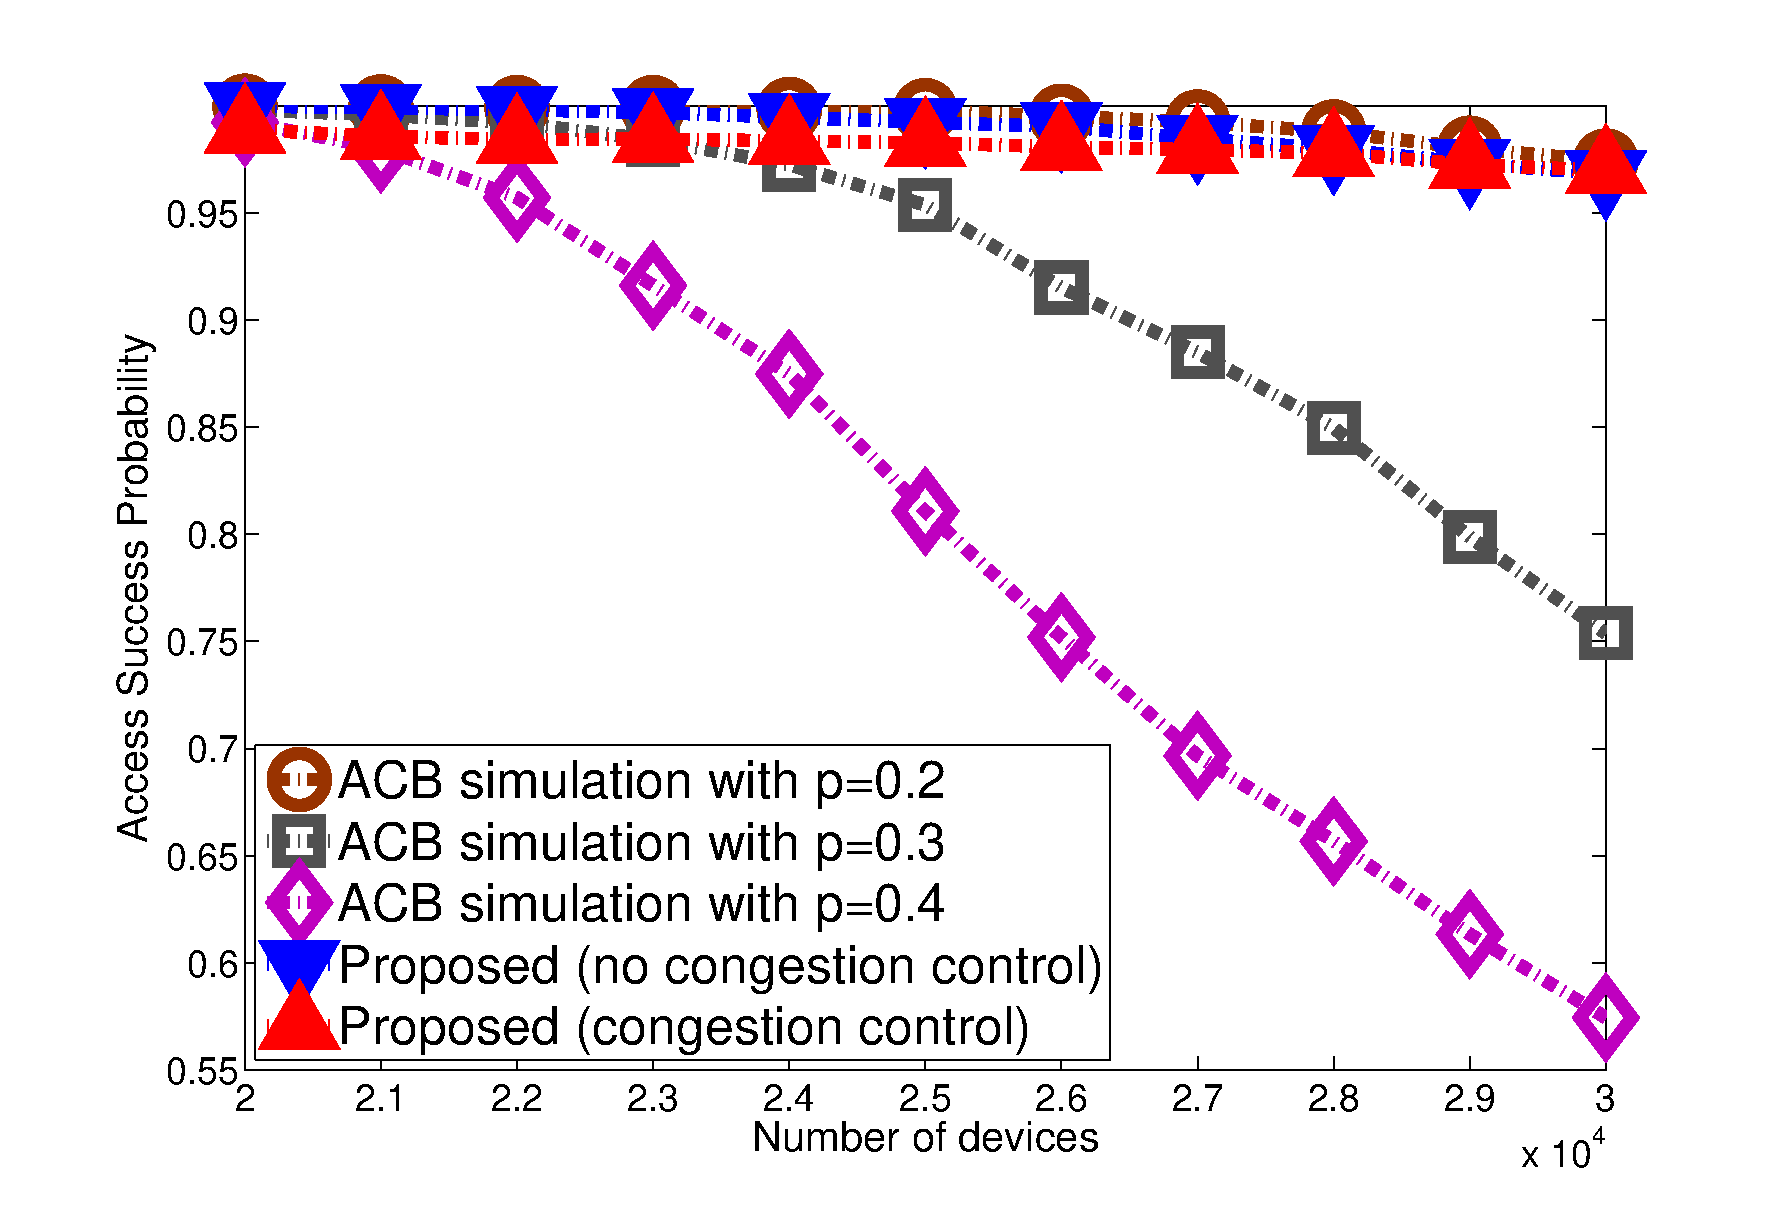
\includegraphics[width=3.8in]{fig_suc_proposed_ACB.eps}
    \caption{Effects of congestion controls and no congestion controls on access success probability}
    \label{fig_suc_proposed_ACB}
    \end{figure}

    \begin{figure}[t]
    \centering
    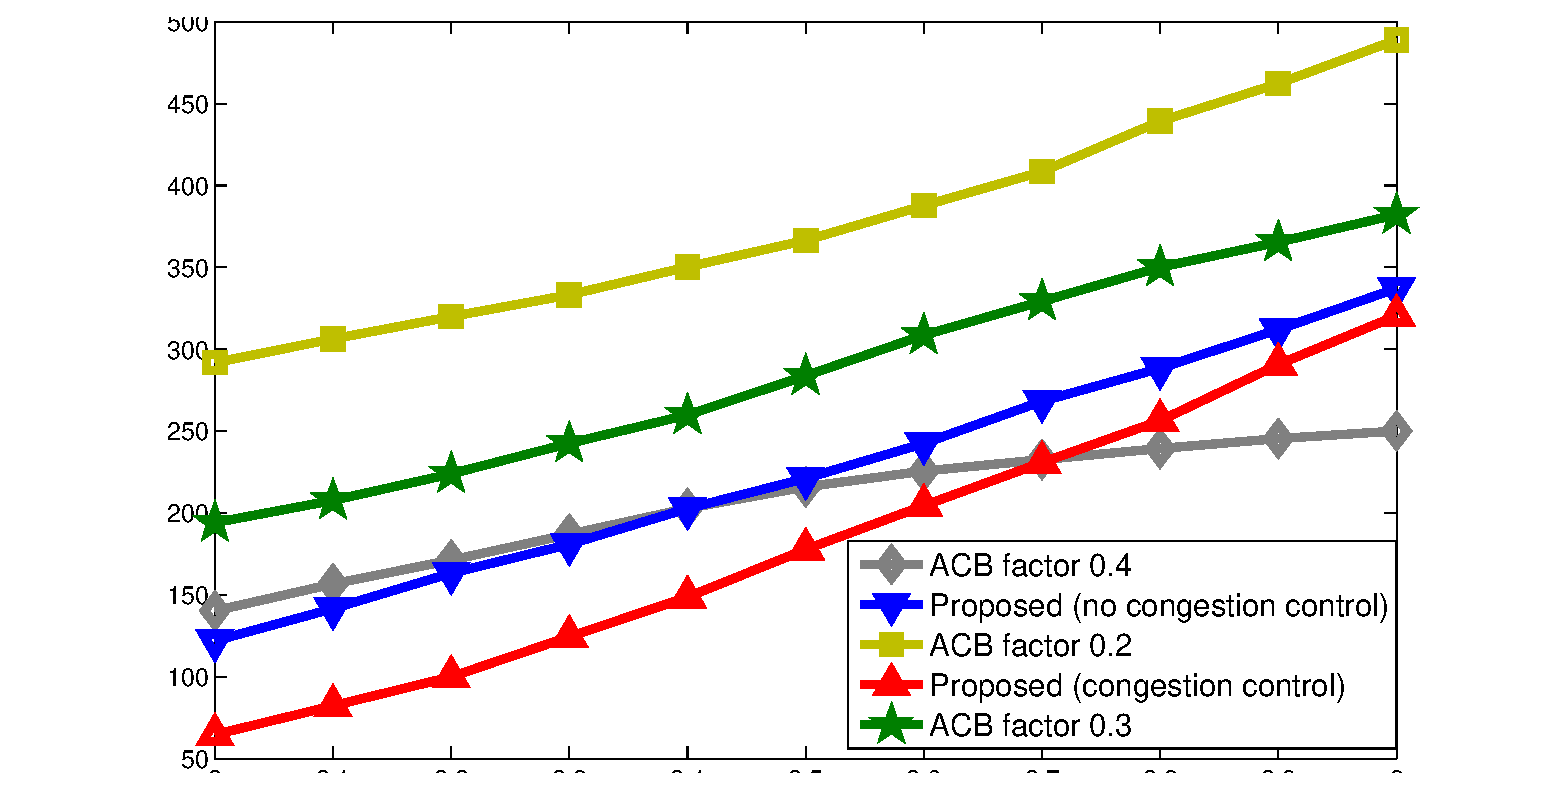
\includegraphics[width=3.8in]{combine_time.eps}
    % 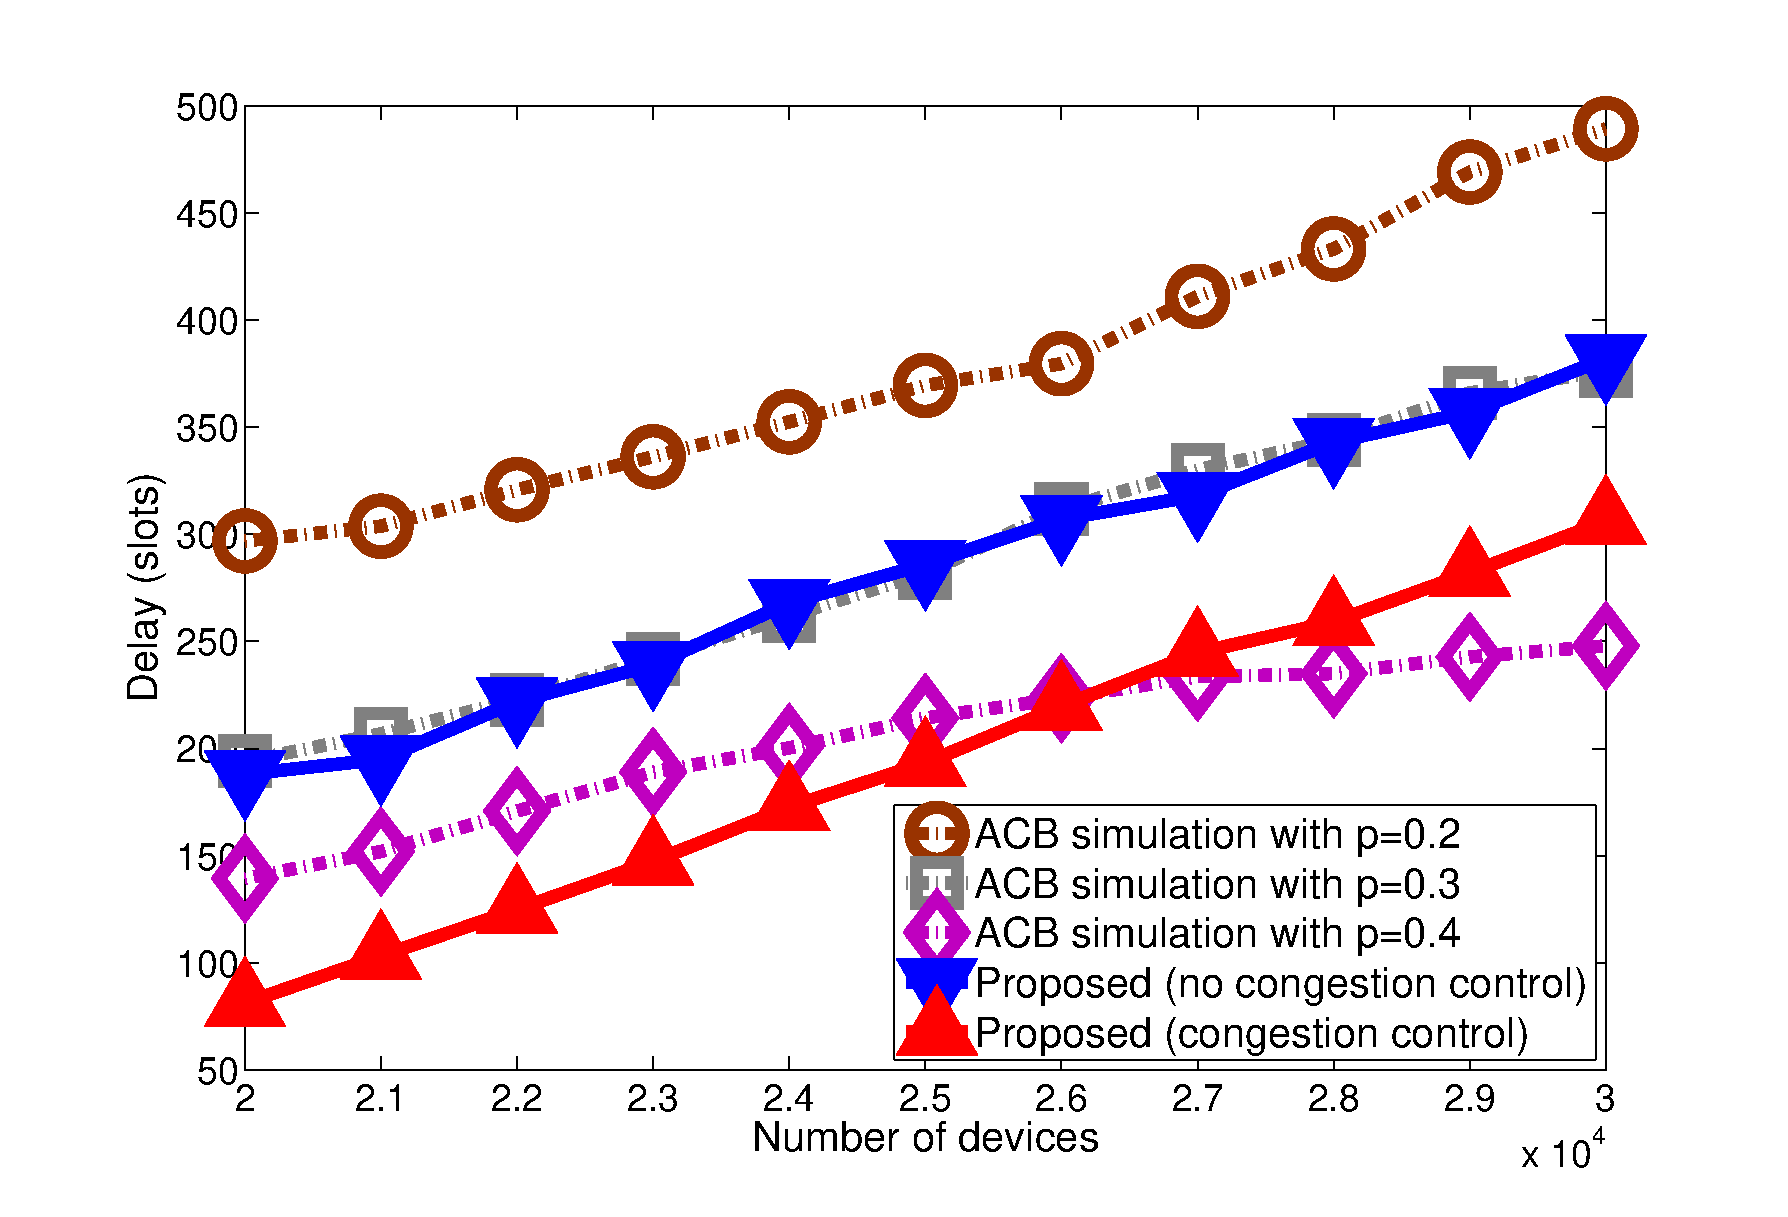
\includegraphics[width=3.8in]{fig_delay_proposed_ACB.eps}
    \caption{Effects of congestion controls and no congestion controls on access success delay}
    \label{fig delay proposed ACB}
    \end{figure}
    Fig.~\ref{fig_suc_proposed_ACB} and Fig.~\ref{fig delay proposed ACB} show the effects of congestion control on access success probability and delay, and the default preamble ratio (weight) of group 1 and gorup2 is $3:7$. We observe that both of the Algorithm 1 and Algorithm 2 have the approximate access success probability, but either Algorithm 1 or Algorithm 2 has the higher access success probability than the traditional ACB scheme with different ACB factor. Obviously, our proposed work can achieve the same access success probability (about 97\%) as the traditional ACB scheme with ACB factor which is equal to $0.2$, but it can reduce delay effectively through congestion control.
    % \begin{figure}[t]
    % \centering
    % 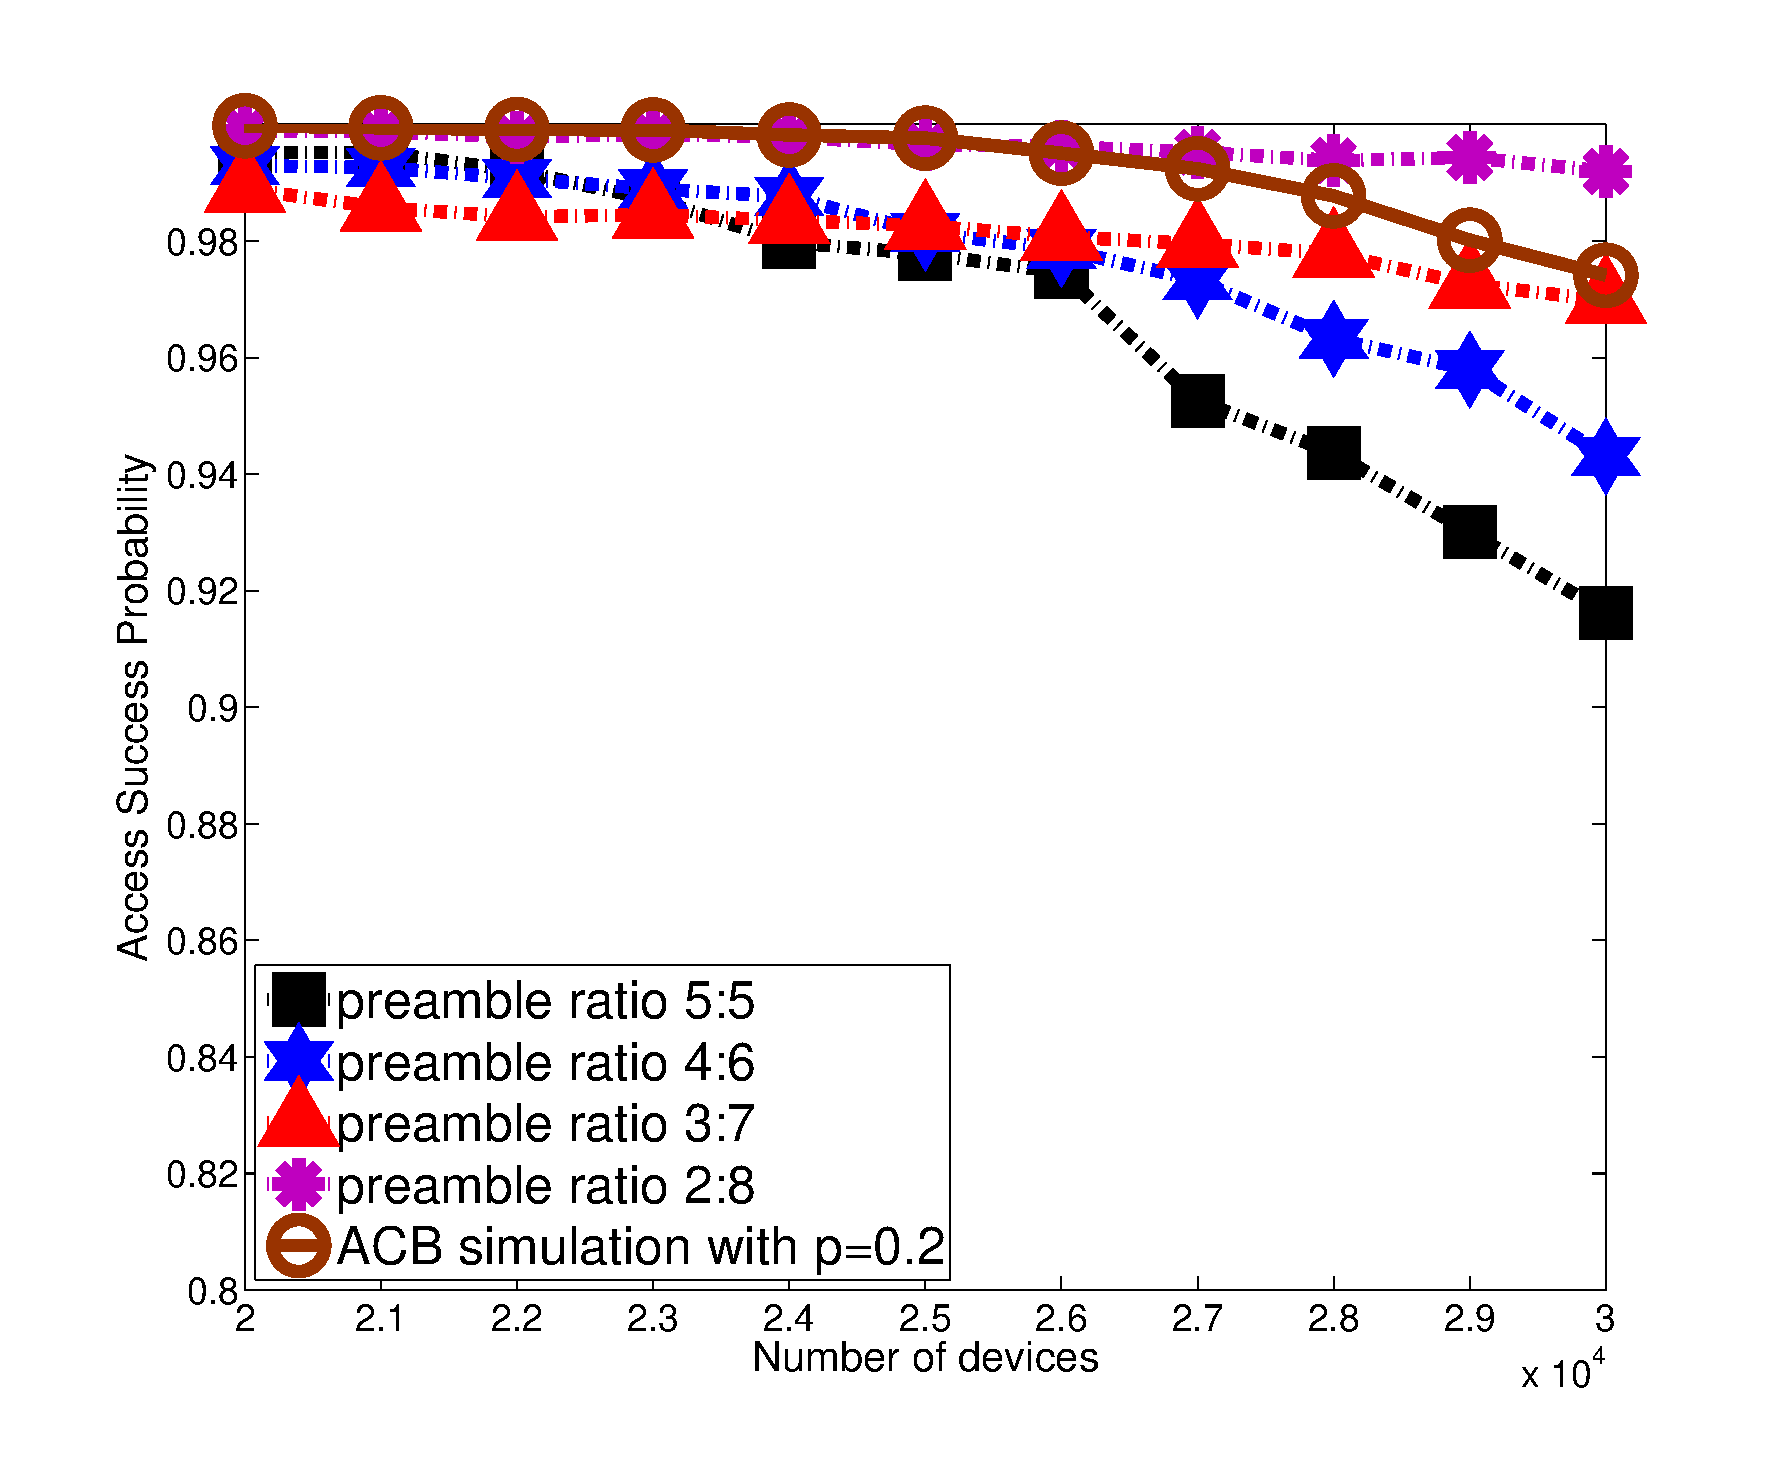
\includegraphics[width=5in]{fig_suc_proportion_congrstion.eps}
    % \caption{Effects of congestion controls and preamble ratio on access success probability}
    % \label{fig_suc_proportion_congrstion}
    % \end{figure}

    % \begin{figure}[t]
    % \centering
    % 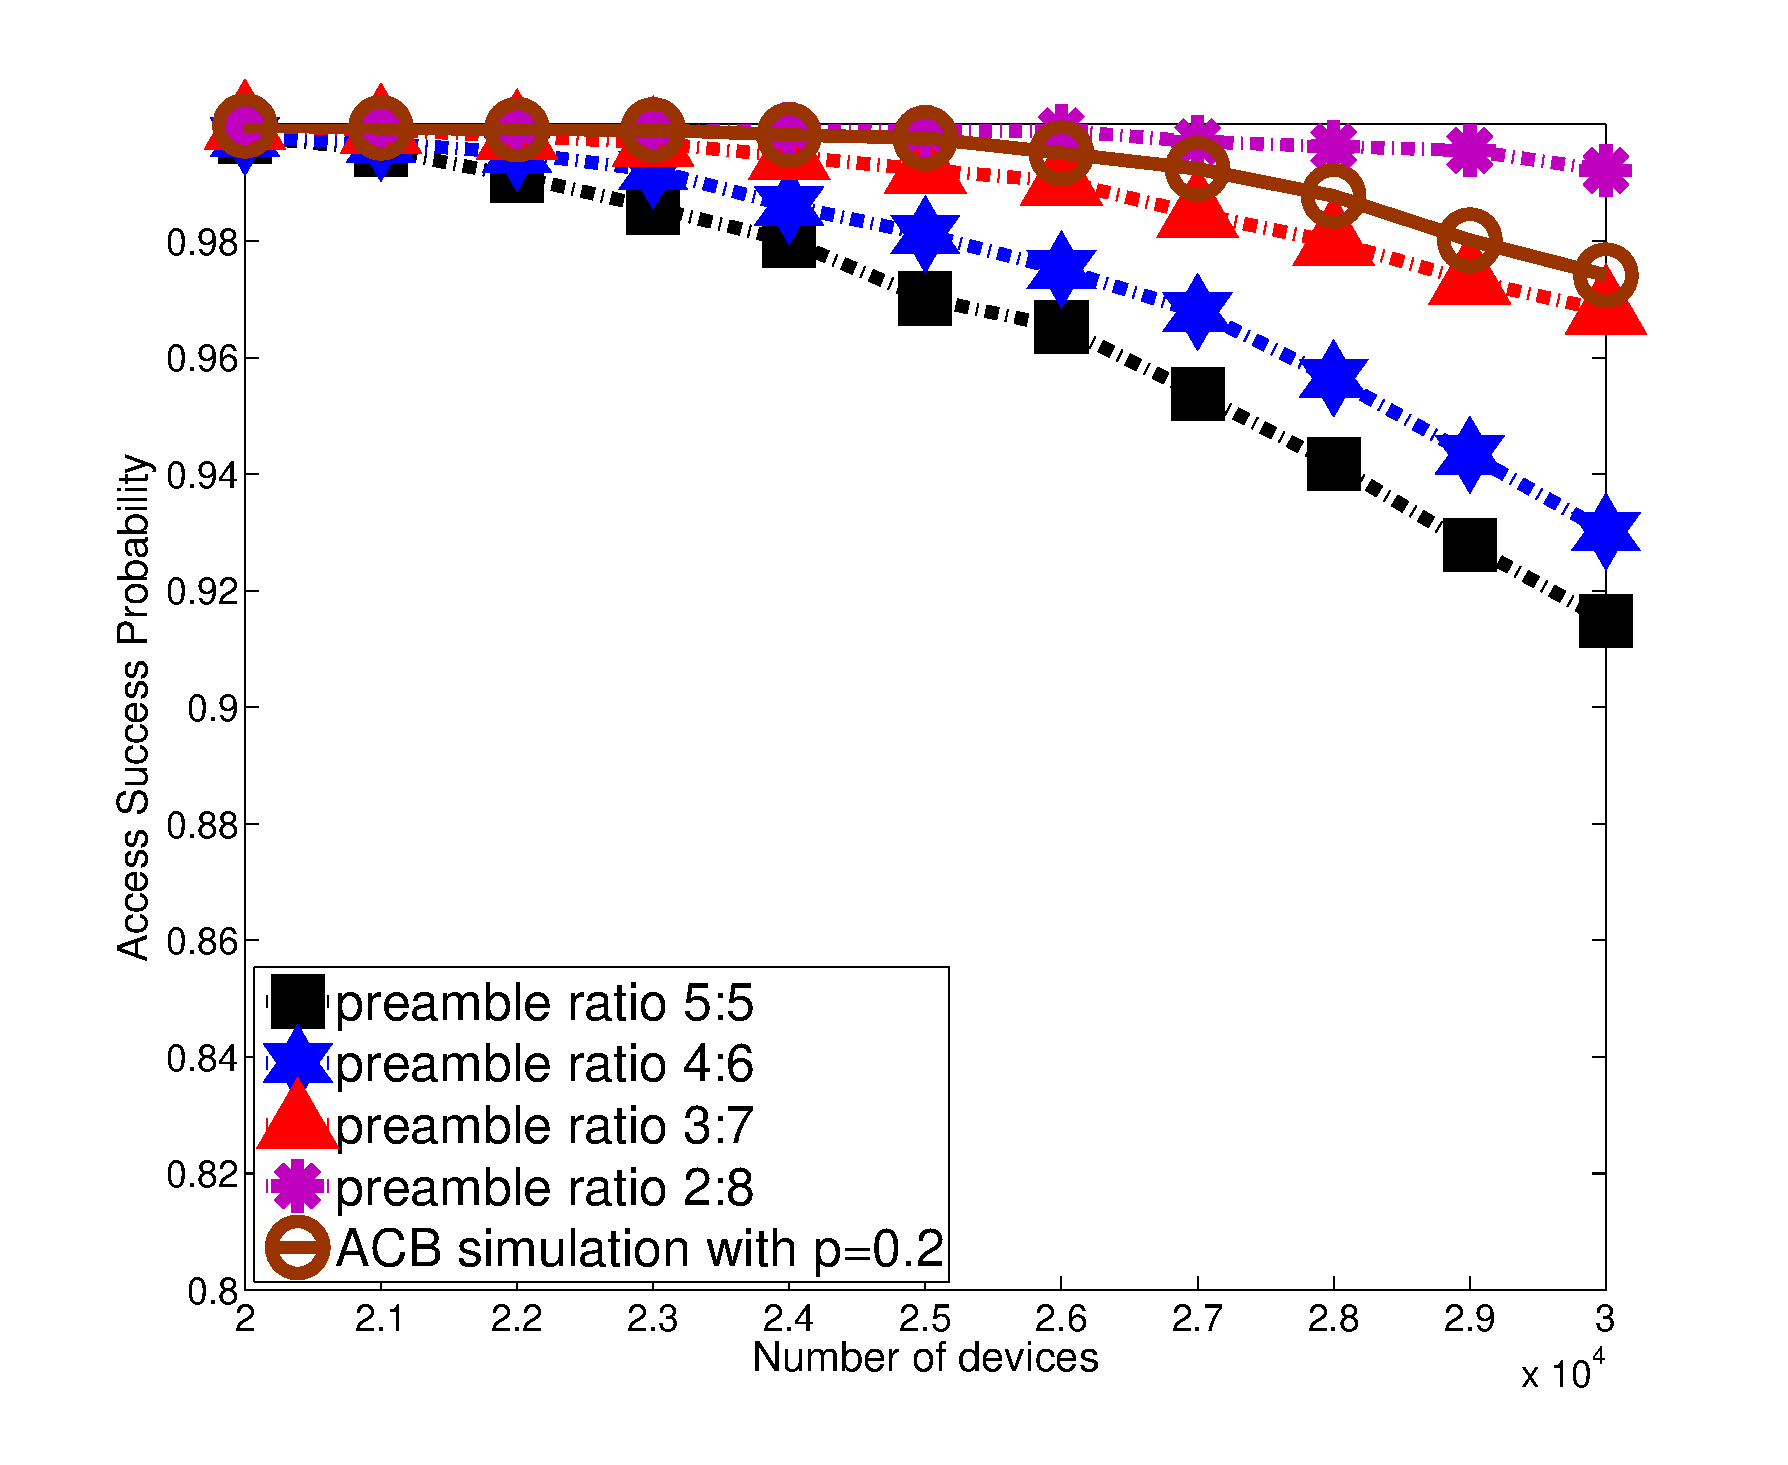
\includegraphics[width=5in]{fig_suc_proportion_no_congrstion.eps}
    % \caption{Effects of no congestion controls and preamble ratio on access success probability}
    % \label{fig_suc_proportion_no_congrstion}
    % \end{figure}

    % \begin{figure}[t]
    % \centering
    % 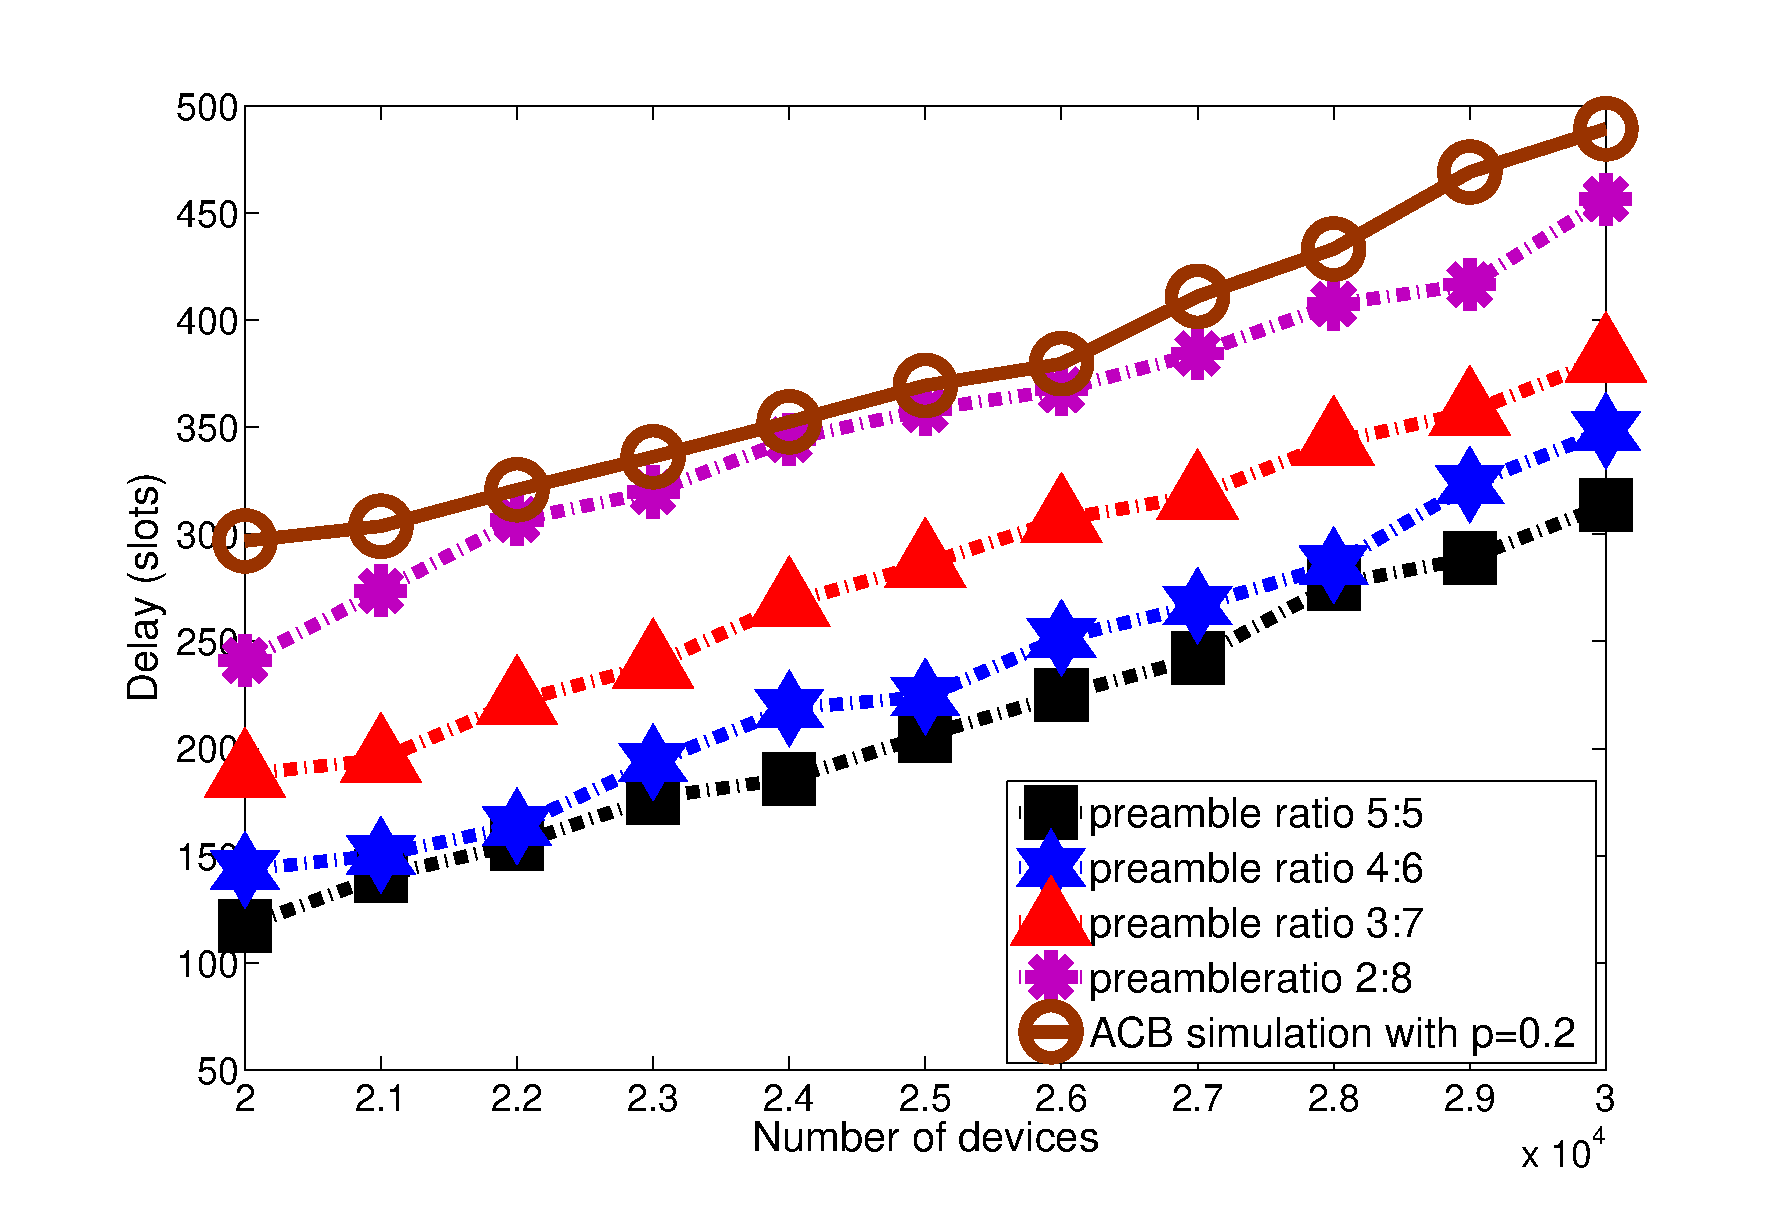
\includegraphics[width=5in]{fig_delay_proportion_no_congrstion.eps}
    % \caption{Effects of no congestion controls and preamble ratio on delay.}
    % \label{fig_delay_proportion_no_congrstion}
    % \end{figure}

    % \begin{figure}[t]
    % \centering
    % 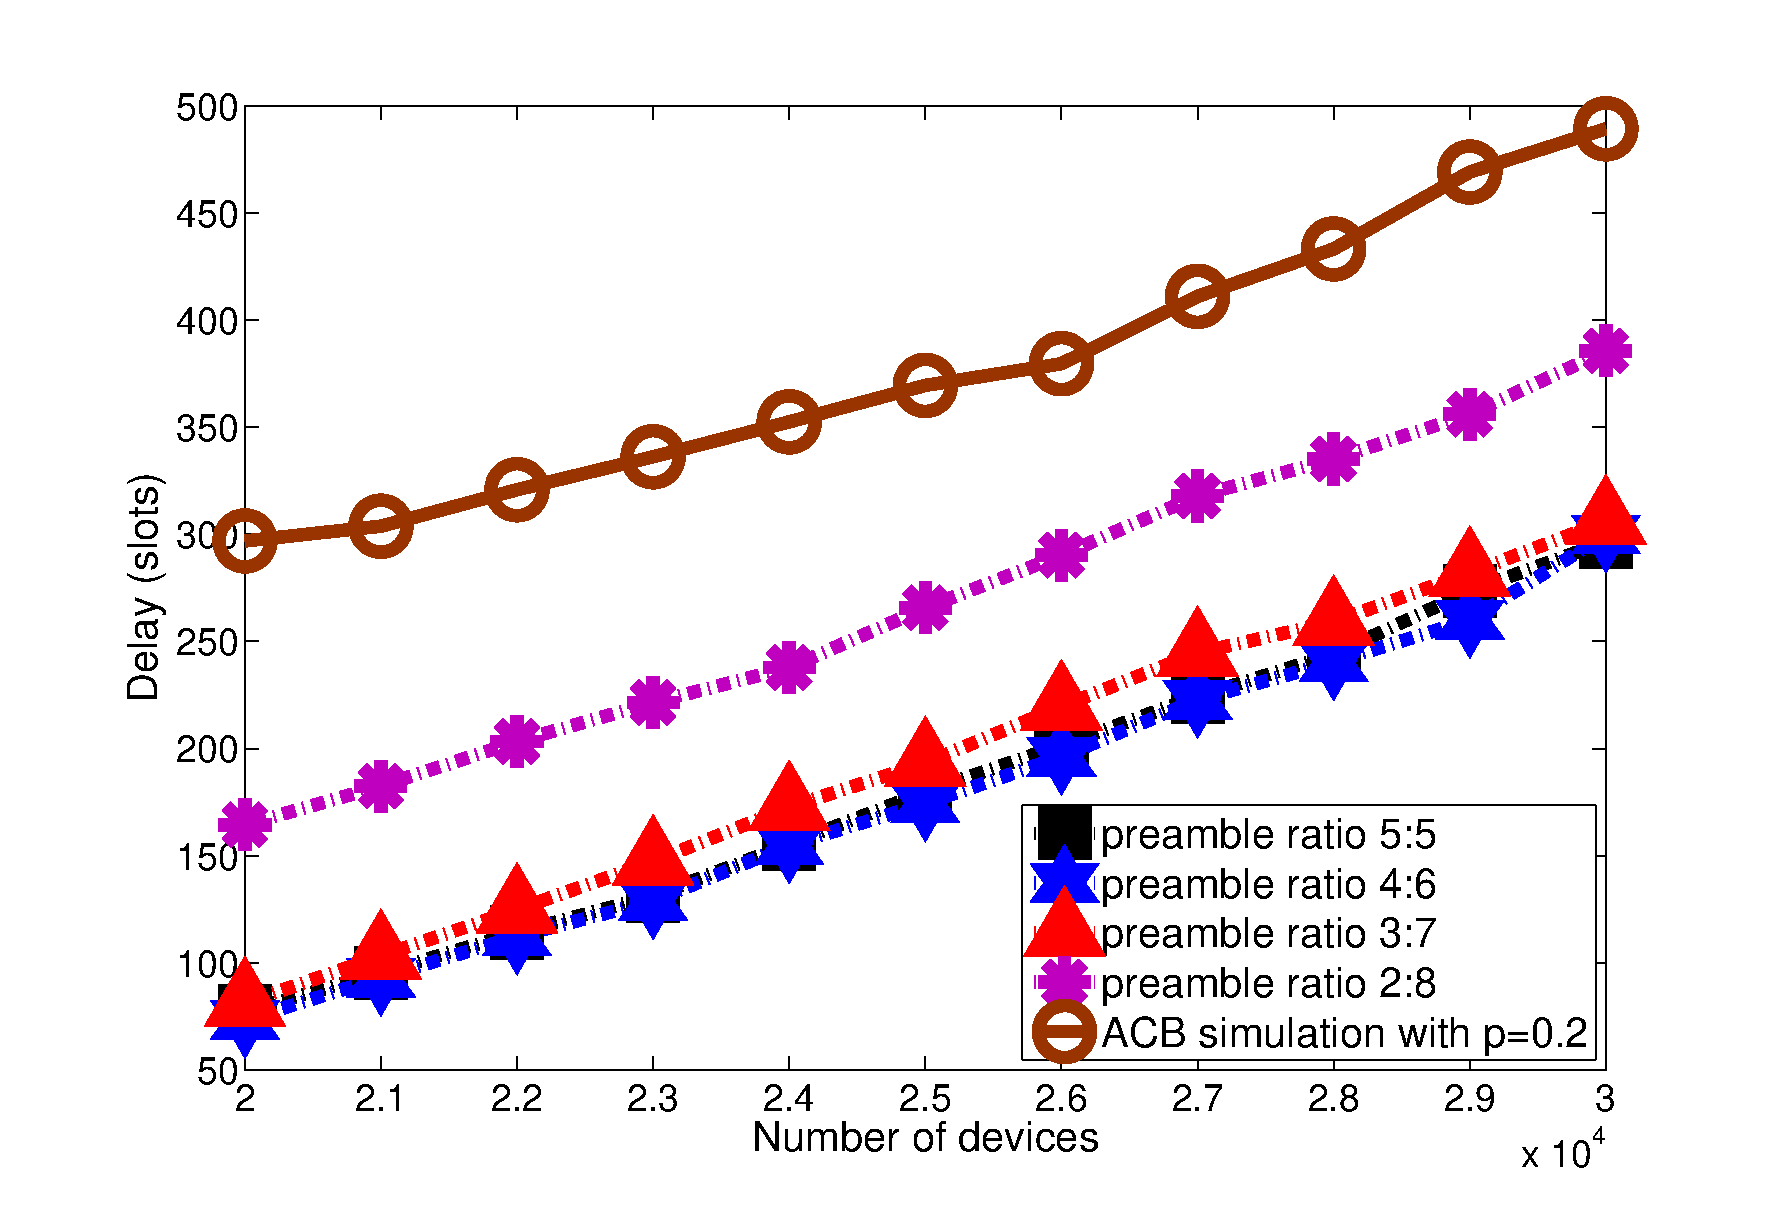
\includegraphics[width=5in]{fig_delay_proportion_congrstion.eps}
    % \caption{Effects of congestion controls and preamble ratio on delay.}
    % \label{fig_delay_proportion_congrstion}
    % \end{figure}
    % Fig.~\ref{fig_suc_proportion_congrstion} and Fig.~\ref{fig_suc_proportion_no_congrstion} show the effects of congestion controls and preamble ratio on access success probability. According to above results, if we assign group 2 the higher preamble ratio, those MTC devices, whose number of preamble transmissions is close to the maximum allowable transmissions, will be given a higher access probability to access the network in order to avoid being expelling from the random access procedure. Therefore, the access success probability is getting better due to the reason that we can efficiently decrease the devices who may fail in the random access procedure. Moreover, the payoff of promoting the access success probability is the heavy delay shown in Fig.~\ref{fig_delay_proportion_no_congrstion} and Fig.~\ref{fig_delay_proportion_congrstion}.
    % \begin{figure}[t]
    % \centering
    % 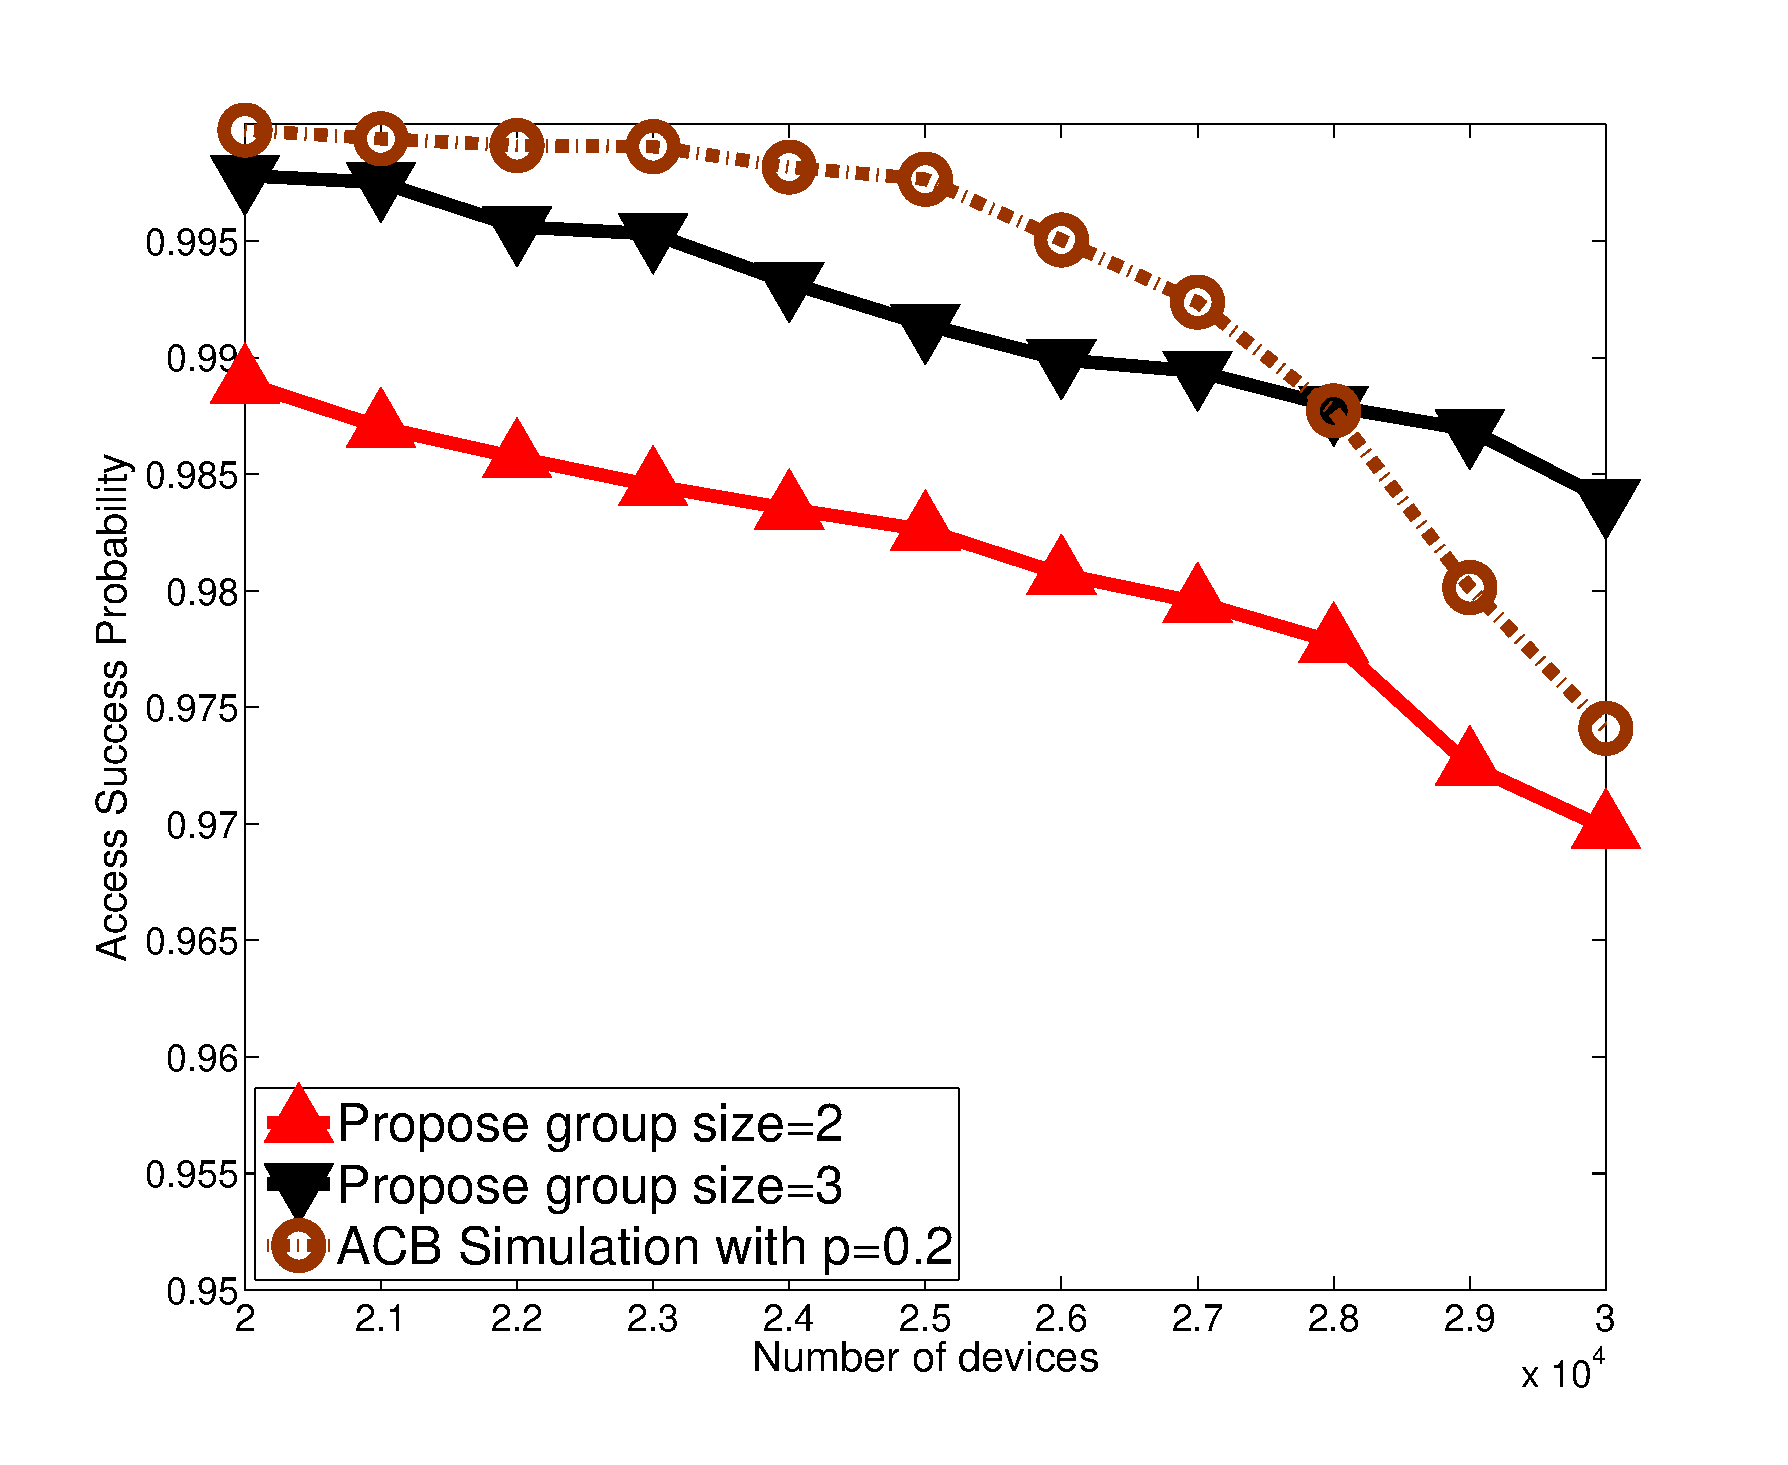
\includegraphics[width=5in]{fig_suc_group_3.eps}
    % \caption{Effects of group size on access success probability}
    % \label{fig_suc_group_3}
    % \end{figure}

    % \begin{figure}[t]
    % \centering
    % 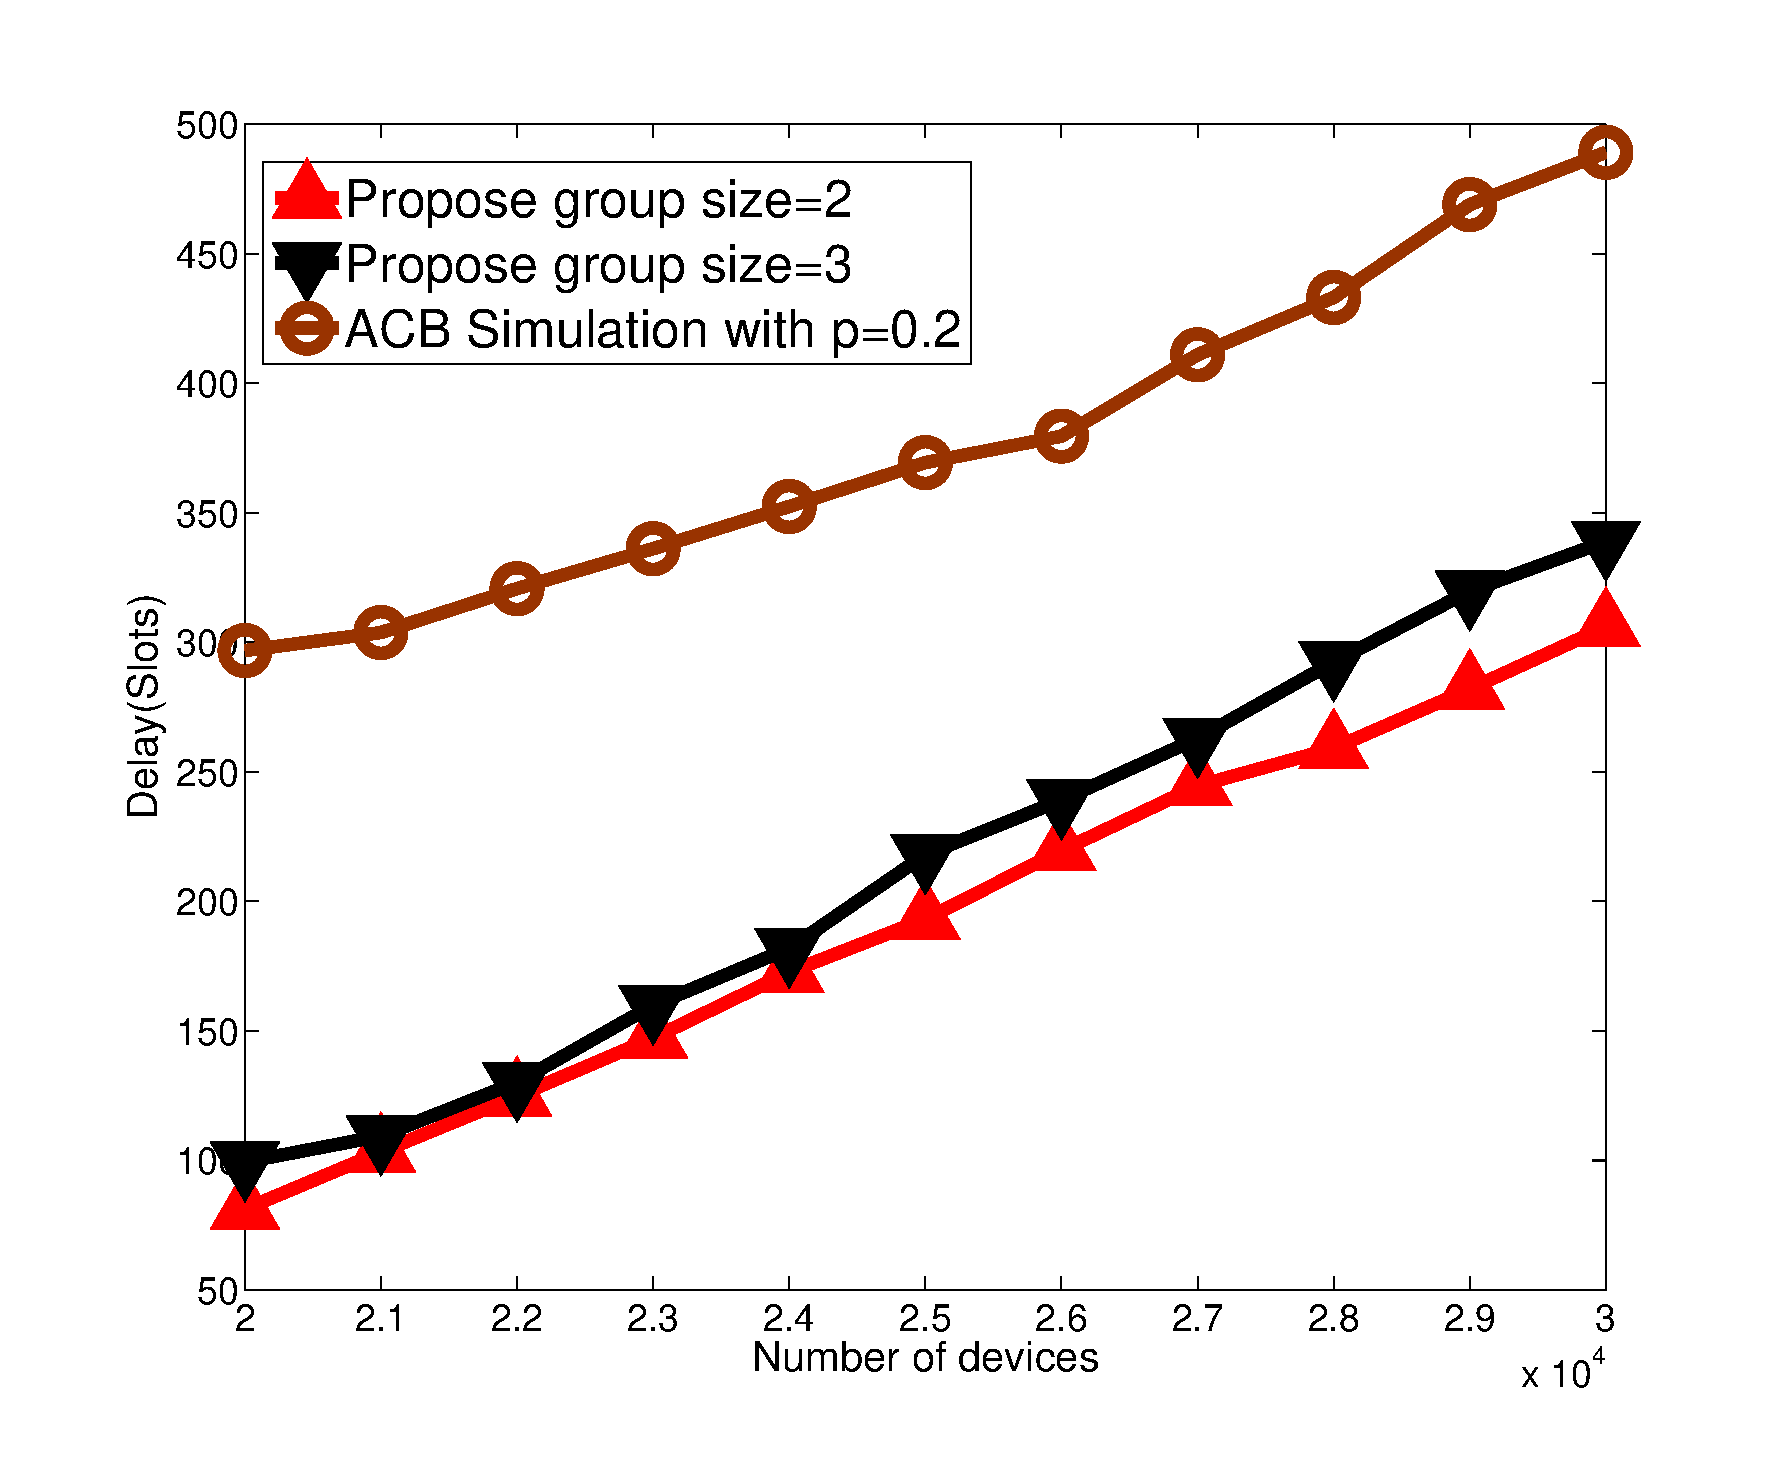
\includegraphics[width=5in]{fig_delay_group_3.eps}
    % \caption{Effects of group size on access success delay}
    % \label{fig_delay_group_3}
    % \end{figure}
    % Fig.~\ref{fig_suc_group_3} and Fig.~\ref{fig_delay_group_3} show the effects of group size on access success probability and delay. When we add the group size, the performance of access success probability is getting higher. However, delay is getting worse when we add the group size due to the reason that the low priority groups have to wait other groups who own the higher priorities so that they may raise the average delay in the system. 